\subsubsection{Inserimento di un utente}
Il diagramma di sequenza rappresenta l'azione di inserimento di un esercizio nel sistema
\begin{figure}[H]
\centering
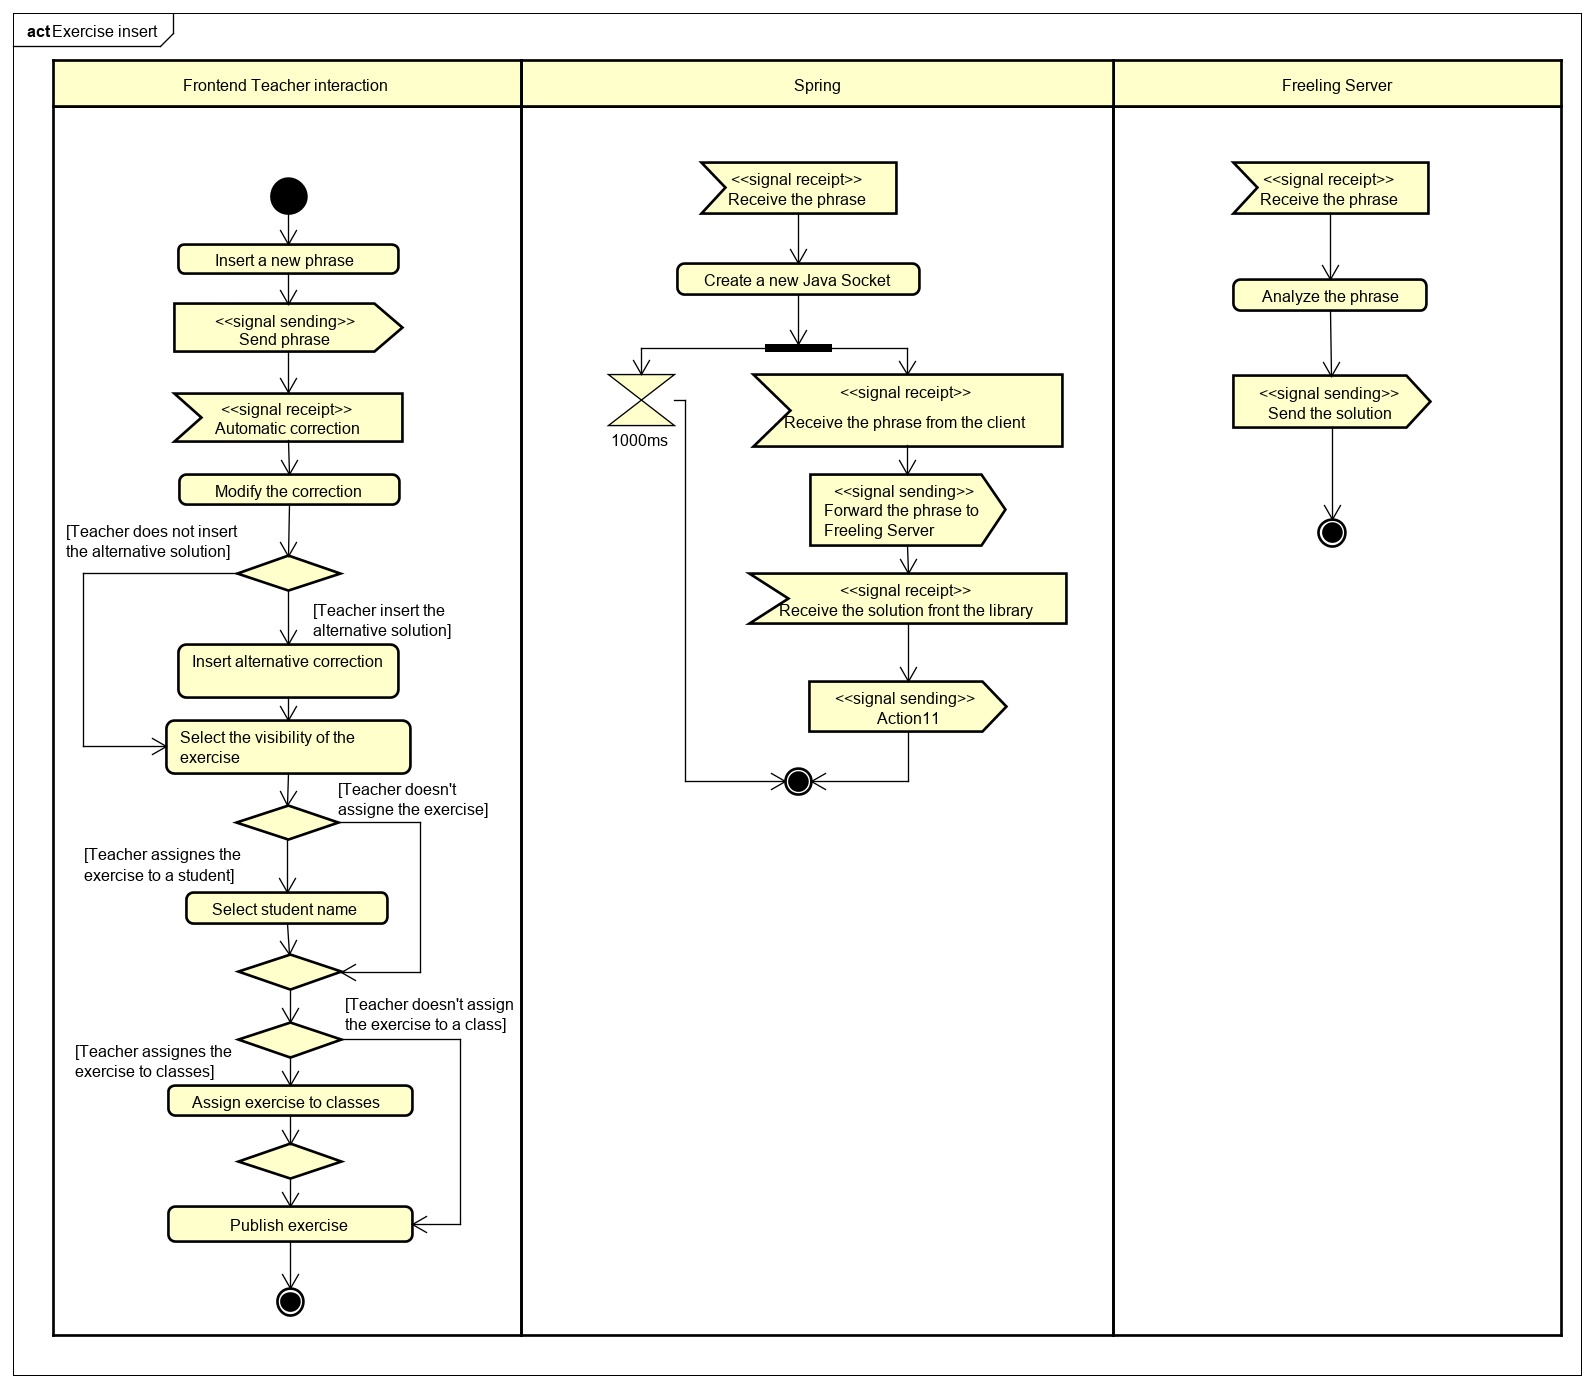
\includegraphics[width=17cm, keepaspectratio]{img/Exercise-insert.png} 
\caption{Exercise insert}
\end{figure}

\begin{figure}[H]
\centering
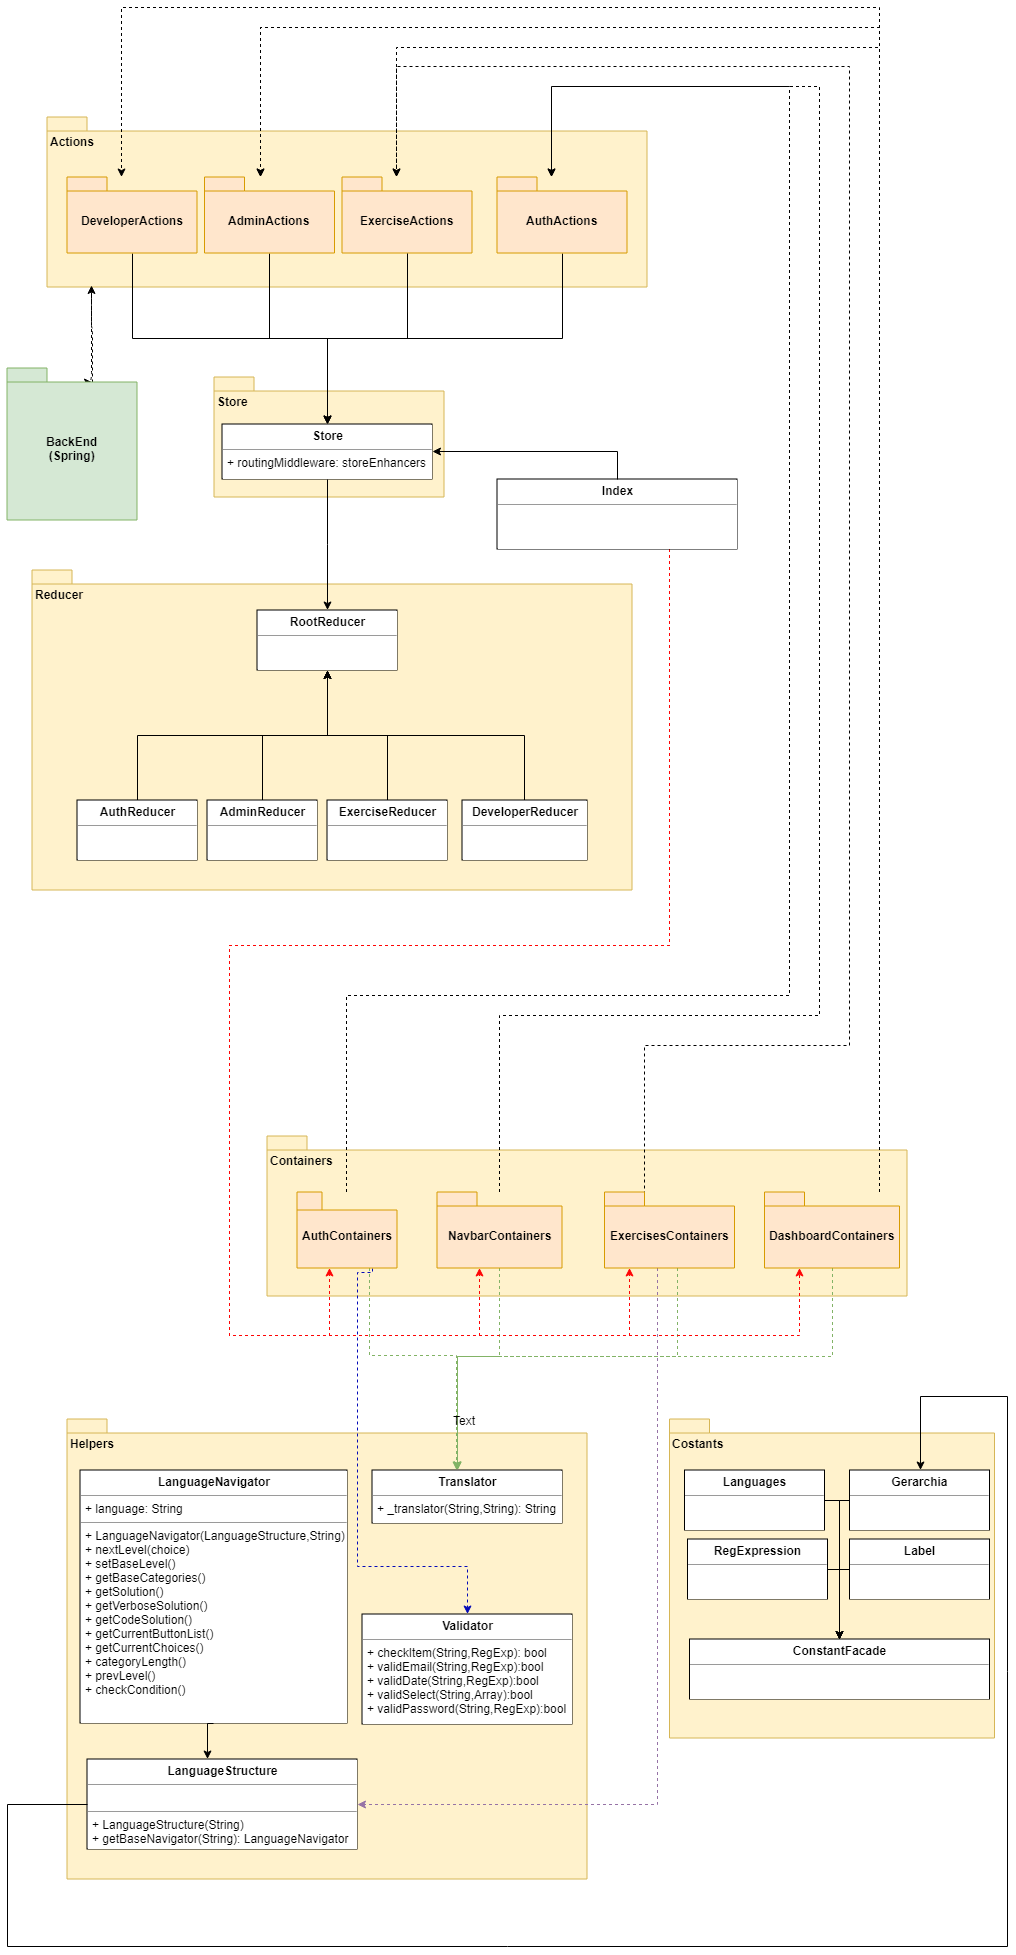
\includegraphics[width=18cm, height=23cm]{img/ReactSpec1.png} 
\caption{UML - FrontEnd}
\end{figure}

\subsubsection{Login}
Il diagramma di sequenza riportato qui di seguito raffigura il processo di login, durante il quale l'utente che vuole accedere può essere autenticato dal sistema.
\begin{figure}[H]
\centering
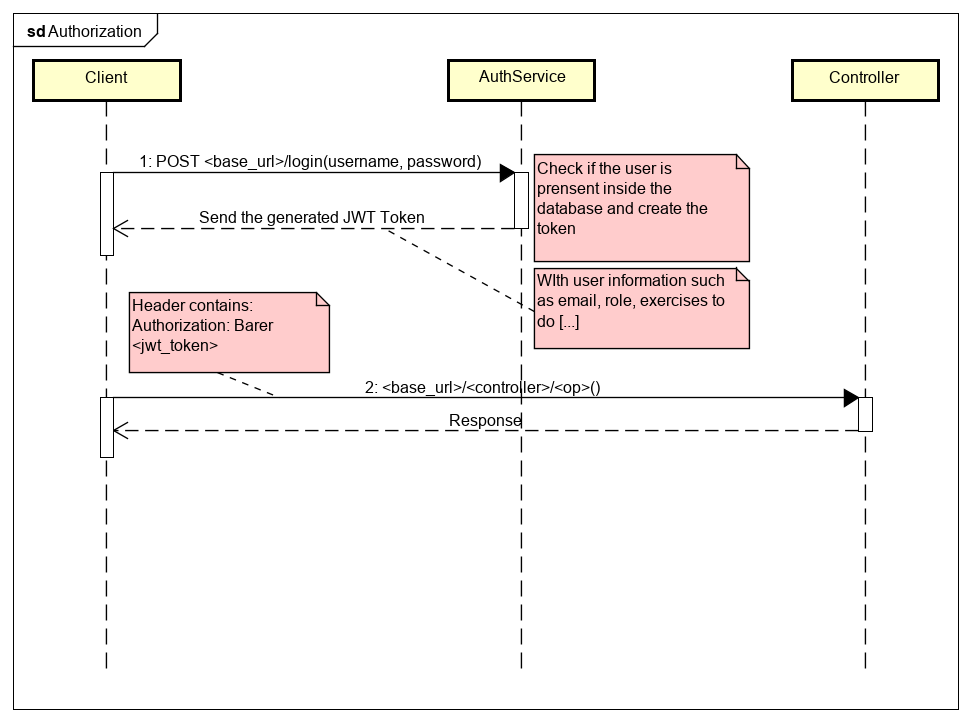
\includegraphics[width=17cm, keepaspectratio]{img/Authorization.png} 
\caption{Authorization}
\end{figure}

